\documentclass{beamer}
\usepackage[utf8]{inputenc}

\usetheme{Madrid}
\usecolortheme{default}
\usepackage{amsmath,amssymb,amsfonts,amsthm}
\usepackage{txfonts}
\usepackage{tkz-euclide}
\usepackage{listings}
\usepackage{adjustbox}
\usepackage{array}
\usepackage{tabularx}
\usepackage{gvv}
\usepackage{lmodern}
\usepackage{circuitikz}
\usepackage{tikz}
\usepackage{graphicx}

\setbeamertemplate{page number in head/foot}[totalframenumber]

\usepackage{tcolorbox}
\tcbuselibrary{minted,breakable,xparse,skins}



\definecolor{bg}{gray}{0.95}
\DeclareTCBListing{mintedbox}{O{}m!O{}}{%
  breakable=true,
  listing engine=minted,
  listing only,
  minted language=#2,
  minted style=default,
  minted options={%
    linenos,
    gobble=0,
    breaklines=true,
    breakafter=,,
    fontsize=\small,
    numbersep=8pt,
    #1},
  boxsep=0pt,
  left skip=0pt,
  right skip=0pt,
  left=25pt,
  right=0pt,
  top=3pt,
  bottom=3pt,
  arc=5pt,
  leftrule=0pt,
  rightrule=0pt,
  bottomrule=2pt,
  toprule=2pt,
  colback=bg,
  colframe=orange!70,
  enhanced,
  overlay={%
    \begin{tcbclipinterior}
    \fill[orange!20!white] (frame.south west) rectangle ([xshift=20pt]frame.north west);
    \end{tcbclipinterior}},
  #3,
}
\lstset{
    language=C,
    basicstyle=\ttfamily\small,
    keywordstyle=\color{blue},
    stringstyle=\color{orange},
    commentstyle=\color{green!60!black},
    numbers=left,
    numberstyle=\tiny\color{gray},
    breaklines=true,
    showstringspaces=false,
}
%------------------------------------------------------------

\title
{2.6.34}
\author 
{AI25BTECH11023 - Pratik R}



\begin{document}


\frame{\titlepage}
\begin{frame}{Question}
\centering
Find the area of region bounded by the triangle whose vertices are $(-1, 1)$,$(0, 5)$ and
$(3, 2)$.
\end{frame}


\begin{frame}[fragile]
    \frametitle{Theoretical Solution}
Given: $A(-1,1),\; B(0,5),\; C(3,2).$\\

$
\vec{B}-\vec{A} =\myvec{1\\4},\qquad
\vec{C}-\vec{A} = \myvec{4\\1}.
$\\

$\norm{\vec{(B-A)} \times \vec{(C-A)}} = \norm{\,\myvec{|\vec{A_{11}} & \vec{B_{23}}| \\ |\vec{A_{31}} & \vec{B_{31}}| \\ |\vec{A_{12}} & \vec{B_{12}}|}\,} = 15 $\\\\


$
\text{Area}=\frac{1}{2}\norm{\vec{(B-A)} \times \vec{(C-A)}} = 7.5
$

\begin{align}
    \centering
    \boxed{Area \, of \, Triangle \, ABC \,= \,7.5\,sq.units}
\end{align}
\end{frame}

\begin{frame}{Graph}
   \centering
    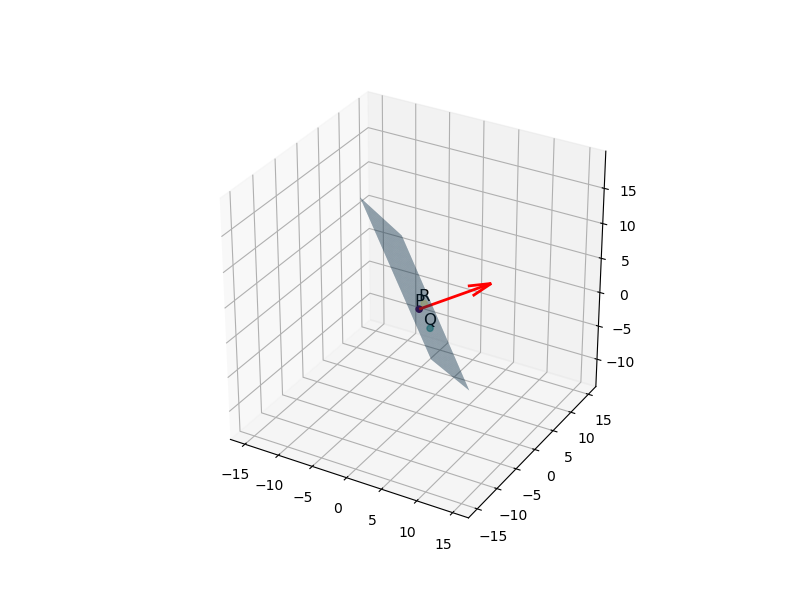
\includegraphics[width=\columnwidth, height=0.8\textheight, keepaspectratio]{figs/fig.png}
    \label{fig:Beamer/figs/fig.png}
\end{frame}


\end{document}